\begin{center}
  \Large
  \textbf{BIOGRAFI PENULIS}
\end{center}

\addcontentsline{toc}{chapter}{BIOGRAFI PENULIS}

\vspace{2ex}

\begin{wrapfigure}{L}{0.3\textwidth}
  \centering
  \vspace{-3ex}
  % Ubah file gambar berikut dengan file foto dari mahasiswa
  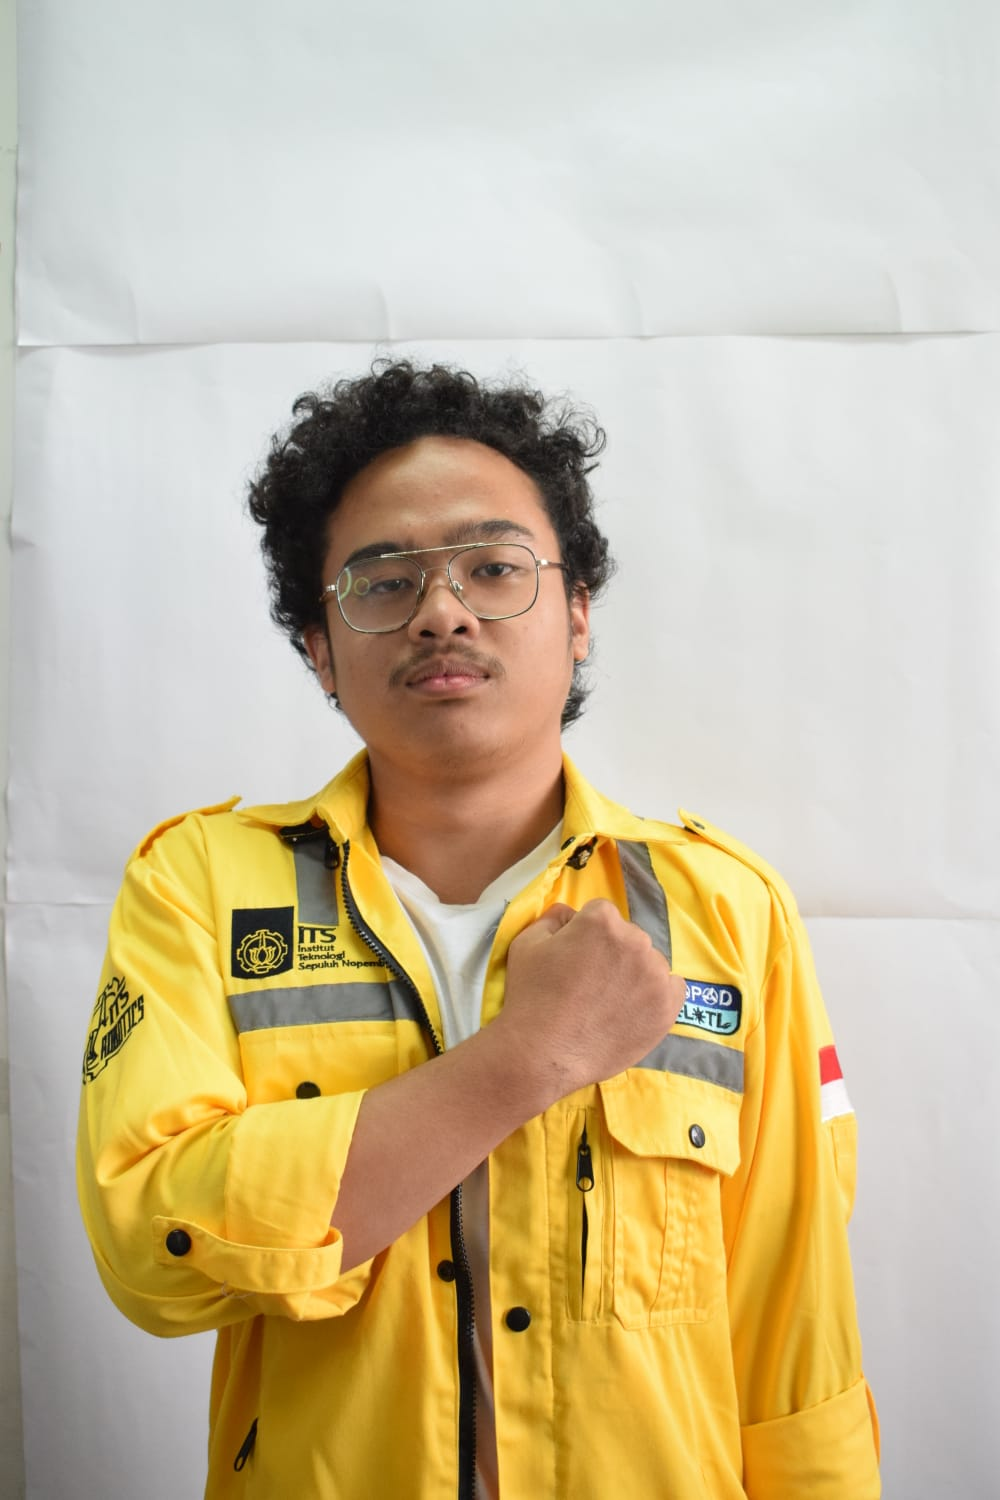
\includegraphics[width=0.3\textwidth]{BiografiPenulis/foto.jpeg}
  \vspace{-4ex}
\end{wrapfigure}

% Ubah kalimat berikut dengan biografi dari mahasiswa
Penulis bernama \name{}, lahir di Sukabumi pada tanggal 14 Februari 2004. Penulis menempuh pendidikan terakhir di SMA Pesantren Unggul AL-Bayan. Ketertarikan penulis terhadap dunia teknologi telah mendorongnya untuk mendalami bidang robotika, kecerdasan buatan. Pada tahun 2022, penulis melanjutkan pendidikan tinggi pada Program Studi Sarjana (S1) Teknik Komputer, Departemen Teknik Komputer, Fakultas Teknologi Elektro dan Informatika Cerdas, Institut Teknologi Sepuluh Nopember (ITS).

Selama masa studi di perguruan tinggi, penulis merupakan mahasiswa yang sangat aktif dan berprestasi, baik dalam riset, kompetisi, maupun pengembangan karier profesional. Penulis tergabung sebagai staf ahli divisi pemrograman dalam tim riset robot bawah air Banyubramanta ITS. Bersama tim ini, penulis turut berkontribusi dalam merancang kontrol dan sistem otonom AUV yang membuahkan hasil membanggakan, di antaranya Juara 1 Nasional Kontes Robot Bawah Air Indonesia (KRBAI) 2024 dan Juara 1 MATE ROV ASEAN 2023.

Di luar lingkup kompetisi, penulis juga aktif mengasah keterampilan teknisnya melalui program magang sebagai \emph{AI Engineer Intern} di PT. Altimeda Cipta Visitama, serta memimpin pengembangan Web pada ITS EXPO 2023, serta berkontribusi dalam pengembangan website pada acara MAGE X. Penga\-laman-penga\-laman ini memperkuat keahlian pengembangan perangkat lunaknya, dengan fokus pada membangun sistem backend yang skalabel dan efisien. 

% Penulis saat ini sedang menyusun Tugas Akhir (TA) berjudul ``SISTEM INSPEKSI VISUAL PADA ROBOT \textit{QUADRUPED} BERBASIS \textit{LARGE LANGUAGE MODEL} DENGAN MEKANISME \textit{HU\-MAN-IN-THE-LOOP}'', sebuah inovasi yang mengintegrasikan \textit{Large Language Model} melalui standar \textit{Model Context Protocol} (MCP) untuk memampukan sistem inspeksi dengan penalaran berbasis semantik dalam operasionalnya. Melalui penelitian tersebut, penulis berharap dapat memberikan kontribusi signifikan terhadap perkembangan teknologi robotika berbasis AI di Indonesia. Bagi pembaca yang tertarik untuk berdiskusi, penulis dapat dihubungi melalui email \url{muhamadrizanoalamsyah@gmail.com}.